% comando para correção ortográfica
%$ aspell -t -c introducao.tex --encoding=utf-8 --lang=pt_BR

\chapter{Introdução}

\section{Problemática}
O consumo de jogos é crescente nos últimos 5 anos, como podemos ver na figura
\ref{fig:esa_graph_2017} das pesquisas da ESA,
segundo os mesmos, em 2016 o consumidor norte americano gastou em torno de $30.4$
bilhões de dólares na industria dos jogos. No mesmo ano, as companhias de jogos
norte americanas adicionaram mais de 11.7 bilhões de dólares na \textit{GDP}
do país \cite{entertainment2017essential}.

\begin{figure}[h]
    \captionsetup{justification=raggedright, singlelinecheck=false}
    \centering
    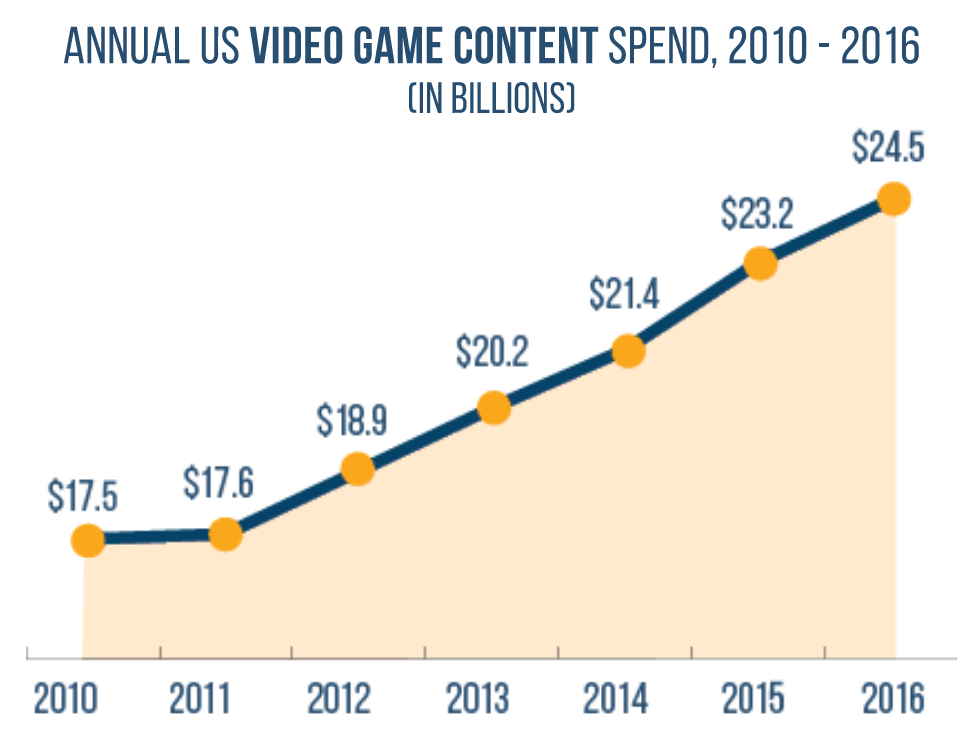
\includegraphics[width=0.5\textwidth]{figuras/ESAGraph2017.png}
    \caption{Consumo com conteúdo de jogos\cite{entertainment2017essential}}
    \label{fig:esa_graph_2017}
\end{figure}

Em contrapartida, os investimentos nos jogos também são crescentes neste
período \cite{entertainment2017essential}, um dos jogos com mais investimentos é
o \textit{GTAV} que em desenvolvimento e marketing gastou cerca de $265$
milhões de dólares \cite{villapaz2013gta}. Os jogos tendem a ser cada vez mais,
detalhados e complexos, desta maneira o custo de desenvolvimento também aumenta.
No desenvolvimento de jogos temos vários profissionais envolvidos para criar
o conteúdo dos jogos, com equipes de programadores, designers,  roteiristas,
entre outros. A força de trabalho dos mesmos costuma ser a parte mais cara da
criação do jogo.


\section{Apresentação}
Uma maneira de conseguir diminuir os gastos no desenvolvimento de conteúdo, é 
gerando os mesmos proceduralmente, as chamadas técnicas de \textit{PCG}. 
\textit{PCG} é usar algoritmos para gerar o conteúdo \cite{shaker2016procedural}.
Uma aplicação bem comum do \textit{PCG} é a criação de relevos e mapas de altura,
desta maneira não é necessário uma pessoa modelar manualmente a altura do
terreno do cenário.

Com o \textit{PCG} para criar o terreno, é possível criar eles com tamanhos
pseudo-infinitos, hoje temos diversos exemplos de jogos que fazem uso dessa técnica
para criar um cenário pseudo-infinitos, entre eles, \textit{Limit Theory}, nele
são criados pseudo-infinitos sistemas planetários, de forma procedural, e em cada
sistema planetário os planetas e seus relevos também são gerados proceduralmente
\cite{abreu1990toward}.




%\subsubsection{Exemplo de ilustração}

%\begin{figure}[h]
%\captionsetup{justification=raggedright, singlelinecheck=false}
%\centering
%
\includegraphics[scale=0.4]{figuras/uffs.eps}
%\caption{Exemplo de ilustração.}
%\label{fig:uffs}
%\end{figure}



%Exemplo do Matheus
%\begin{figure}[H]
%  \centering
%  \includegraphics[width=0.9\textwidth]{figuras/tcc2/pts_sem_peso/evento_de_site_insercao_fronteiras.png}
%  \caption{ES para o \textit{site} $s$.}
%  \label{fig:cenario_insercao_de_fronteiras}
%\end{figure}
%
%  Levando em consideração o cenário da figura \ref{fig:cenario_insercao_de_fronteiras}, 
%$s$ está contido em $R^{*}_{q}$, portanto serão criadas as fronteiras $C^{-}_{qs}$ e $C^{+}_{qs}$,
